%\subsubsection{Sensor Precision Testing}
%The purpose of this subsubsection is to test the sensors available, to assess their precision and eventual quirks that we should keep in mind during further work. Afterwards we will compare our results to the associated datasheets.
%\todo{Mention our project specific requirements/hypothesis (which doesn't exist yet).}

\subsubsection{Expectations}
We expect that the sensors will be wildly inaccurate, and that we will manually need to include the results of these measurements in further work, in order for it to not hurt the product and its reliability.

\subsubsection{Planning}
We have the following sensors, many of which will need to be tuned to the same input:
1x LEGO Ultrasound Sensor
- Returns 10 bits, corresponding to distance in cm. from an obstacle.
2x LEGO Light Sensor
- Returns a 10 bit unsigned integer describing how much light is picked up by the sensor.

More to be added soon...\todo{Finish writing this.}

\subsubsection{Measurements}
\subsubsection{Ultrasonic Sensor} \label{Analysis:ultrasonicTests}
The Ultrasonic Sensor is build with the purpose of recognize objects, avoid obstacles, measure distances, and detect movement. It does this as the name implies, sending sound waves and calculating the time it takes for that sound wave to hit an object and return back to the sensor by knowing the sound speed.

In figure \ref{NXT-Ultrasonic-Sensor} the ultrasonic sensor can be seen. It consists of two "eyes", a transmitter(left) and a receiver(right)\cite{ExposedLEGOUltrasonic}. 

\begin{figure}[H]
    \centering
    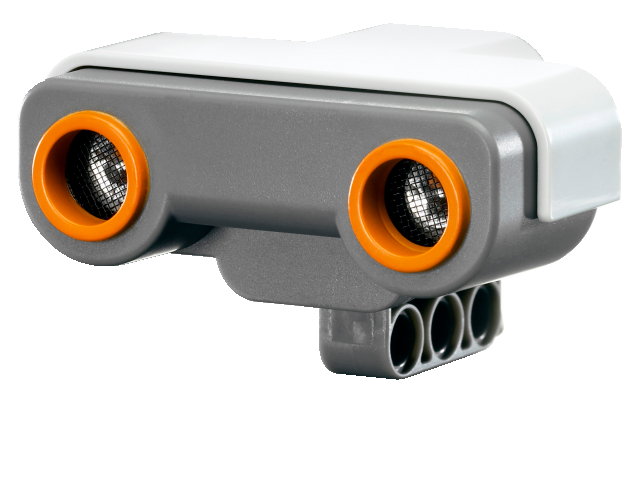
\includegraphics[width=0.5\textwidth]{Images/Analysis/NXT-Ultrasonic-Sensor.png}
    \caption{The ultrasonic sensor: Left eye is the transmitter, and right eye is the receiver.}
    \label{fig:NXT-Ultrasonic-Sensor}
\end{figure}

% Billede http://www.legoengineering.com/wp-content/uploads/2013/04/NXT-Ultrasonic-Sensor.png

The Ultrasonic Sensor measures the distance in centimeters and
inches. The sensor range is 0 to 255 centimeters with a precision of +/-3 cm. But this is with the perfect shape objects, the real range depends on the shape of the object it tries to detect. For example, soft and curved objects like a ball can be hard to detect. While large-sized hard surface  objects like a wall, can be easier to detect\cite{}. Furthermore if the range is 255 it's an indicator the sound wave didn't return in time, and didn't detect any objects.
% https://www.generationrobots.com/media/Lego-Mindstorms-NXT-Education-Kit.pdf




A sound beep does not travel in a narrow straight line. Instead it spreads out like the light beam of a torchlight. As a result the sensor not only detects objects that are exactly in front of the sensor, it also detects objects that are somewhat to the left or right.







result of tests???



The sensor testing chapter can be found in appendix



\ref{ultrasonicSensorTesting}\todo{Add ref to camerasensortesting}.


\subsubsection{Light Sensor}

\subsubsection{Motors}

\subsubsection{Conclusion}
\todo{Write this}